\documentclass[oneside,a4paper,12pt]{book}

\input{estilo.tex}

\makeindex

\usepackage{hyperref}
\usepackage{footmisc}

\usepackage{graphicx}
\usepackage{subcaption}

\usepackage{tabularx}
\usepackage{hyperref}
\usepackage{xurl}
\usepackage{multirow}

\usepackage{amsmath}

\usepackage{makecell}
\usepackage{booktabs}

\begin{document}
\baselineskip 1.35\baselineskip

\frontmatter

\thispagestyle{empty}
\vspace{2cm}

\begin{figure}[htb]
  \hspace{-0.5cm}\centerline{\resizebox{.55\textwidth}{!}{
\includegraphics{figs/logo_urjc.jpg}}}
\end{figure}

\begin{center}
  \vspace{0.7cm}

  \hspace{-1.5cm}{\Large{ESCUELA DE INGENIERÍA DE\\
  \hspace{-1.5cm}\vspace{3mm} FUENLABRADA}}

  \vspace{1.5cm}

  \hspace{-1.5cm}{\Large {GRADO EN\\
  \hspace{-1.5cm}\vspace{3mm} INGENIERÍA DE ROBÓTICA SOFTWARE}}

  \vspace{1.5cm}

  \hspace{-1.5cm}{\Large \bf {TRABAJO FIN DE GRADO}}

  \vspace{1.5cm}

{\large {IMPLEMENTACIÓN DE UN ROBOT POR CABLES PARA EL\\
CONTROL DE UN EFECTOR FINAL EN DIVERSAS TAREAS
}}

  \vspace{3.5cm}

  \hspace{-1.5cm}{\bf Autor}: Alberto León Luengo\\ \vspace{3mm}
  \hspace{-1.5cm}{\bf Tutor}: Dr. Juan Sebastián Cely Gutiérrez \\ \vspace{3mm}

  \vspace{2.5cm}

  \hspace{-1.5cm}{\large {Curso académico 2025-2026}}
\end{center}

\clearpage
\thispagestyle{empty}


\input{portada/licencia.tex}

\cleardoublepage

\chapter*{Agradecimientos}

Me gustaría mostrarles todo mi agradecimiento a mis padres, Natividad y Alberto, que han estado siempre apoyándome en todo momento y ayudándome a superar los obstáculos más difíciles a los que he tenido que hacer frente a lo largo de estos seis años de etapa universitaria.

\vspace{0.25cm}

A mi hermana Ainhoa, por ser capaz de sacarme una sonrisa siempre que la situación no ha sido favorable y por ayudarme a salir de mi rutina habitual manteniéndome dentro de mi zona de confort.

\vspace{0.25cm}

A Juan, mi tutor, por el buen trato y todos los nuevos conocimientos y enseñanzas que he podido aprender gracias a él en todo el tiempo que he compartido con él realizando este TFG.

\vspace{0.25cm}

Y por último, a todos los compañeros que me han estado acompañando en la recta final de este viaje, y que gracias al apoyo que ellos me han ofrecido y que yo de la misma forma les he ofrecido a ellos, todos mis objetivos y éxitos esperados han acabado dando sus frutos.

\thispagestyle{empty}


\cleardoublepage

\chapter*{Acrónimos\markboth{Acrónimos}{Acrónimos}}

\begin{acronym}
    \acro{TFG}{\emph{Trabajo de Fin de Grado}}
	\acro{CDPR}{\emph{Cable Driven Parallel Robot}}
    \acro{ROS}{\emph{Robot Operating System}}
    \acro{RViZ}{\emph{ROS Visualization}}
    \acro{URDF}{\emph{Unified Robot Description Format}}
\end{acronym}


\cleardoublepage

\tableofcontents

\listoffigures

\listofmyequations

\cleardoublepage


\let\OLDthebibliography=\thebibliography
\def\thebibliography#1{\OLDthebibliography{#1}
  \addcontentsline{toc}{chapter}{\bibname}}

\mainmatter

\setcounter{page}{1}
\chapter{Introducción}
\label{cap:capitulo1}
\setcounter{page}{1}

\vspace{0.25cm}

\section{Contexto y motivación}
\label{sec:segundaseccion}

Los robots paralelos accionados por cables, también conocidos como Cable Driven Parallel Robots (CDPR), han despertado bastante interés en los últimos años tanto en el ámbito académico como en el ámbito industrial. Este tipo de robots basa su funcionamiento en el uso de cables que pueden ser recogidos o elongados por poleas con el objetivo de desplazar el efector final que une todos los cables a una posición específica, obteniendo como resultado una estructura ligera, escalable, y lo más importante de todo, capaz de realizar grandes volúmenes de trabajo en comparación con otros tipos de robots.

\vspace{0.25cm}

Durante los últimos seis años, los cuales he dedicado enteramente a mi formación en el Grado en Ingeniería de Robótica Software, y tras haber abordado diferentes campos de la robótica, he decidido decantarme por este tipo de robots como tema principal de mi TFG, ya que combina conceptos de modelado matemático y cinemático, el uso de un lenguaje de programación de alto nivel como lo es Python, y una de las arquitecturas software por excelencia utilizadas en el mundo de la robótica: ROS 2. Este Trabajo de Fin de Grado tiene como objetivo principal la profundización en el diseño y el desarrollo de un CDPR de dos grados de libertad desde un punto de vista práctico y orientado al software.

\begin{figure} [h!]
    \begin{center}
        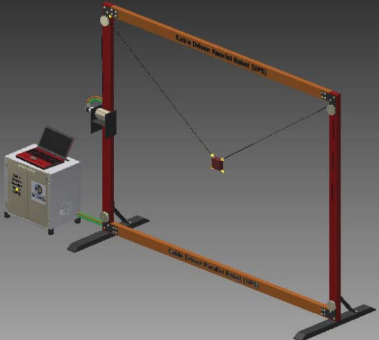
\includegraphics[width=0.5\textwidth]{figs/cdpr_model.png}
    \end{center}
    \caption{Ejemplo visual de un CDPR de dos grados de libertad}
\end{figure}\

\newpage

Y por último, es importante mencionar que la principal motivación que me ha llevado a elegir este tipo de robots como tema principal de mi TFG es que el comportamiento global del sistema viene determinado principalmente por la correcta formulación del modelo cinemático, además de todo lo que respecta a la implementación software.

\section{Planteamiento del problema}
\label{sec:segundaseccion}

El problema principal que se aborda en este TFG es el control de la posición de un efector final suspendido mediante dos cables ubicados en una estructura fija, en este caso una pizarra móvil con ruedas, a través de poleas, donde el sistema debe ser capaz de desplazar el efector final hacia una o varias posiciones específicas, siendo capaz de definir trayectorias en caso de que el efector final pase por más de una posición, todo ello dentro de una región bidimensional cuadrada cuya área cuadrada viene definida por la distancia que separa ambas poleas.

\vspace{0.25cm}

Sabiendo esto, es necesario establecer una relación entre la región por la que se mueve el efector final y las variables físicas del sistema, como por ejemplo las longitudes de los cables y el ángulo que debe rotar cada polea para desplazar el efector final a una posición específica. Esta relación debe ser lo suficientemente robusta de forma que pueda implementarse en un entorno real, y lo suficientemente flexible como para poder integrarla en software robótico.

\newpage

En este TFG me he centrado principalmente en desarrollar todo el software necesario para resolver este problema, dejando la implementación del sistema real como una fase posterior, actualmente en proceso de definición y que abordaré en conjunto con mi tutor de TFG, \href{https://github.com/juanscelyg}{Juan Sebastián Cely Gutiérrez}.

\section{Objetivos}
\label{sec:segundaseccion}

El objetivo principal de este TFG consiste en el diseño, implementación y validación de un sistema capaz de controlar un CDPR bidimensional, comenzando por la definición del modelo cinemático, pasando por su integración en ROS 2 y finalizando con la construcción de un prototipo del sistema en un entorno real utilizando elementos hardware.

\vspace{0.25cm}

En términos específicos, los objetivos a destacar son los siguientes:

\begin{itemize}
\item Desarrollo de un modelo cinemático que relacione la posición en la que se encuentre el efector final con las longitudes de los cables y los ángulos de giro de las poleas en cada momento.
\item Validación del modelo desarrollado en distintos lenguajes de programación.
\item Implementación del modelo cinemático en un nodo ROS 2 que ofrezca información sobre el movimiento y las trayectorias realizadas en cada momento.
\item Integración completa del sistema en ROS 2 utilizando RViZ como herramienta de visualización.
\item Integración del software desarrollado en un sistema hardware real.
\end{itemize}

\section{Alcance y limitaciones}
\label{sec:segundaseccion}

El alcance de este TFG se centra principalmente en la parte software del sistema, dentro de la cual se ha desarrollado y validado un modelo cinemático, además de su integración en ROS 2. Sin embargo, no se ha profundizado en otros aspectos como el modelado de fuerzas, las tensiones de los cables, la estructuración del sistema de forma que este sea de tipo ”lazo cerrado”, o una interacción más detallada con los sensores en el sistema real, ya que en este caso, éste está compuesto por dos servomotores como únicos elementos hardware.

\newpage

Por tanto, aunque se presente una descripción del sistema hardware, tanto la construcción del robot real como su puesta en funcionamiento quedan algo más apartadas. Todas estas limitaciones han sido asumidas desde el principio, ya que otro de los objetivos principales de este TFG comprende que toda la parte del desarrollo software sea sólida.

\section{Metodología}
\label{sec:segundaseccion}

La metodología de este TFG ha sido iterativa e incremental en función de las fases que se han ido abordando. En primer lugar, se ha llevado a cabo la formulación del modelo cinemático del sistema para su posterior validación en pruebas realizadas en diferentes lenguajes de programación como han sido MATLAB, Python y C++ respectivamente, lo que ha permitido detectar y corregir pequeños errores de planteamiento de forma que no se acarreasen hasta fases más avanzadas. Una vez validado el modelo cinemático, se ha procedido a su integración en ROS 2, donde se ha desarrollado un nodo capaz de generar trayectorias y visualizarlas a través de RViZ, lo que ha permitido mantener una separación clara entre validación, simulación e integración.

\section{Descripción inicial del sistema}
\label{sec:segundaseccion}

Aunque la parte hardware del sistema se encuentre en una fase preliminar, se ha planteado un diseño consistente en consonancia con el modelo software desarrollado, en el que el sistema está compuesto principalmente por una estructura rígida,  en este caso una pizarra móvil con ruedas, que soporta dos poleas fijas ubicadas en las esquinas superiores de la misma, a las cuales se conectan los cables encargados de desplazar el efector final.

\vspace{0.25cm}

El movimiento de las poleas se lleva a cabo utilizando servomotores, cuyo tipo y características serán determinados en fases posteriores de este TFG, así como el diseño del efector final y el resto de materiales empleados, los cuales se detallarán una vez finalizada la fase de construcción del sistema real.


\chapter{Fundamentos teóricos}
\label{cap:capitulo2}

\vspace{0.25cm}

\section{Introducción}
\label{sec:segundaseccion}

Los robots paralelos accionados por cables (CDPR) han experimentado un gran crecimiento en los últimos años. Comprenden conceptos de robótica paralela, modelado geométrico y mecánica ligera, convirtiéndolos en un tipo de robots muy atractivo tanto para proyectos de investigación como para aplicaciones prácticas.

\vspace{0.25cm}

Este capítulo presenta el contexto teórico que comprende este TFG, además de abordar conceptos fundamentales sobre los CDPR, sus configuraciones más habituales y sus principales líneas de investigación, todo ello relacionado con el enfoque software adaptado.

\section{Robots paralelos accionados por cables (CDPR)}
\label{sec:segundaseccion}

Un CDPR se caracteriza por utilizar cables como elementos para transmitir el movimiento entre la estructura y el efector final. Esta característica introduce una serie de particularidades desde el punto de vista del modelado y del control del sistema, ya que es necesario garantizar que los cables permanezcan tensionados en todo momento. A pesar de ello, este tipo de robots tiene un peso estructural mucho menor, una mayor escalabilidad y la posibilidad de desplazarse por regiones bastante amplias.

\section{Configuraciones típicas}
\label{sec:segundaseccion}

Los CDPR pueden adoptar múltiples configuraciones en función del número de cables, puntos de anclaje y grados de libertad por los que se mueve el efector final. En caso de que se quiera mover el efector final en tres dimensiones, el número de cables debe ser superior al número de grados de libertad, con el fin de garantizar que todos los cables utilizados se encuentren tensionados.

\vspace{0.25cm}

En este caso, el efector final se mueve en dos dimensiones, por lo que el número de cables debe ser como mínimo igual al número de grados de libertad, condición que se cumple satisfactoriamente desde el principio.

\section{Modelo cinemático}
\label{sec:segundaseccion}

El modelo cinemático de un CDPR tiene como objetivo establecer una relación entre la posición del efector final y las longitudes de los cables que lo accionan en cada momento, todo ello haciendo uso de las distancias euclídeas entre cada polea y el efector final.

\vspace{0.25cm}

En este caso, se ha optado por trabajar directamente con la cinemática inversa, ya que lo que se quiere es calcular las longitudes de cada cable siendo conocida la posición del efector final en cada momento. Este enfoque resulta adecuado para su posterior implementación software e integración en ROS 2.

\section{Control y planificación de trayectorias}
\label{sec:segundaseccion}

El control de un CDPR presenta diversos retos en lo que respecta a los cables y a la contínua necesidad de mantenerlos en tensión, ya que en sistemas más avanzados, lo más habitual es incorporar un modelo dinámico, un sistema de control en lazo cerrado y otras estrategias centradas en la tensión de los cables.

\vspace{0.25cm}

Sin embargo, al tratarse de una aplicación mucho más sencilla, en la que el objetivo principal consiste en la validación del comportamiento geométrico del sistema, lo normal es utilizar un modelo cinemático y un sistema de control en lazo abierto, donde la planificación de trayectorias se realice a partir de un conjunto de posiciones objetivo y los cálculos necesarios para pasar por todas ellas de forma contínua.

\section{Frameworks robóticos}
\label{sec:segundaseccion}

ROS 2 se considera actualmente como uno de los frameworks de referencia en el desarrollo de sistemas robóticos, ya que su arquitectura basada en nodos, topics y servicios, hacen mucho más fácil y llevadera la creación de este tipo de sistemas.

\vspace{0.25cm}

Es por eso que la integración de un CDPR en ROS 2 permite separar y distinguir sin ningún problema el modelo cinemático, la lógica de control y la visualización del sistema simulado, la cual se llevará a cabo en RViZ.

\section{Aplicaciones y líneas de investigación actuales}
\label{sec:segundaseccion}

Los CDPR son utilizados en la actualidad desde sistemas de posicionamiento, manipulación de grandes cargas y plataformas de movimiento, hasta algunos robots de rehabilitación.

\vspace{0.25cm}

Por otro lado, las principales líneas de investigación actuales están centradas en el análisis del espacio de trabajo, la optimización de las tensiones de los cables que componen el sistema, lograr una mayor robustez en el control del sistema y garantizar una interacción segura en todo su entorno.

\section{Relación con el trabajo de fin de grado desarrollado}
\label{sec:segundaseccion}

Este TFG se sitúa dentro de todo este contexto desde un enfoque simplificado en comparación con aplicaciones ya existentes, haciendo énfasis en el desarrollo software, el modelo cinemático y la integración en ROS 2, lo que permite sentar unas bases sólidas de forma que, en un futuro, se pueda añadir un modelo dinámico, el uso de otro tipo de sensores aparte de los servomotores que actúan como poleas, o la implementación de un sistema de control mucho más avanzado.


\chapter{Plataforma de desarrollo}
\label{cap:capitulo3}

\vspace{0.25cm}

\section{Introducción}
\label{sec:segundaseccion}

En este capítulo se presenta una visión global del sistema desarrollado en este TFG, ofreciendo una descripción del CDPR diseñado y de toda la arquitectura que hace posible su funcionamiento, la cual ha permitido validar el modelo cinemático, así como los algoritmos para planificar trayectorias utilizados y su integración en ROS 2. Y aunque gran parte del sistema hardware se encuentre en una fase preliminar, todo su diseño se está teniendo en cuenta desde el principio.

\section{Funcionamiento de un CDPR bidimensional}
\label{sec:segundaseccion}

El funcionamiento principal de un CDPR bidimensional consiste en el desplazamiento de un efector final, dentro de una región del mismo tipo que el robot, todo ello mediante el accionamiento de dos cables, donde cada uno de ellos conecta el efector final con dos poleas fijas, situadas en cada una de las esquinas superiores de la estructura, lo que permite controlar su posición en función de la longitud de cada uno de los cables.

\vspace{0.25cm}

Desde un punto de vista funcional, el sistema recibe como entrada una o varias posiciones objetivo, a partir de las cuales el sistema va calculando las longitudes de los cables y los ángulos de rotación de cada polea necesarios para hacer que el efector final pase por todas y cada una de las posiciones recibidas.

\section{Arquitectura}
\label{sec:segundaseccion}

La arquitectura del sistema sigue un enfoque modular y escalable. Esto significa que, aunque toda su implementación abarque un único nodo, posee un diseño que separa las diferentes capas que componen el sistema, las cuales se describen a continuación:

\begin{itemize}
\item \textit{Capa de entrada}: Define la posición o conjunto de posiciones (trayectorias) objetivo por las que el efector final debe pasar.
\item \textit{Capa cinemática}: Aplica el modelo cinemático para transformar las posiciones recibidas en parámetros físicos del sistema.
\item \textit{Capa visual}: Muestra el estado del sistema en cada momento, lo que permite analizar su comportamiento y comprobar que todo está funcionando correctamente.
\end{itemize}

Toda esta arquitectura facilita la comprensión del sistema y hace que, en caso de que se quiera realizar una ampliación del mismo en un futuro, ésta se pueda llevar a cabo de una forma mucho más sencilla.

\vspace{0.25cm}

Con el objetivo de visualizar el sistema descrito anteriormente, se adjunta a continuación un diagrama que representa la arquitectura general del sistema y la relación entre sus componentes principales.

\begin{figure} [h!]
    \begin{center}
        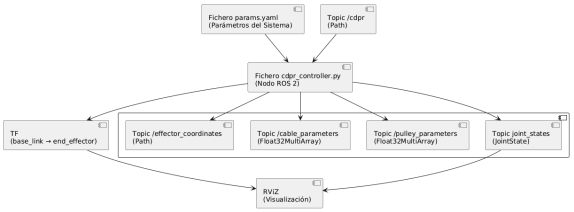
\includegraphics[width=\textwidth]{figs/general_system_architecture.png}
    \end{center}
    \caption{Arquitectura general del sistema en ROS 2}
\end{figure}\

Como se puede observar, se tiene una única posición o un conjunto de posiciones objetivo definidas por el usuario, las cuales se envían al nodo principal del sistema implementado, encargado de aplicar el modelo cinemático del robot para calcular las longitudes y los ángulos respecto a la vertical de cada cable, al igual que los ángulos de rotación y la cantidad de cable elongada o recogida por cada polea.

\newpage

Una vez calculados estos parámetros, toda esta información se publica mediante topics, lo que permite a otros componentes del sistema poder utilizar esta información, mientras se visualiza en RViZ el estado del sistema en cada momento utilizando el modelo URDF definido, lo que permite observar el comportamiento de todos los elementos que componen el sistema durante la ejecución de una trayectoria.

\section{Componentes software}
\label{sec:segundaseccion}

El desarrollo software es lo que compone en su gran mayoría al núcleo de este TFG, el cual se ha llevado a cabo en Python, ya que es un lenguaje de programación de alto nivel que se integra perfectamente con ROS 2 y que se caracteriza principalmente por su flexibilidad y legibilidad en código, siendo éstos los factores principales que he tenido en cuenta a la hora de elegir este lenguaje de programación antes que otros, como han sido MATLAB o C++.

\vspace{0.25cm}

El sistema software está compuesto principalmente por los siguientes elementos, los cuales trabajan de forma coordinada con el objetivo de ofrecer una simulación bastante coherente:

\begin{itemize}
\item Un nodo ROS 2 encargado de gestionar la ejecución del sistema, el cual recibe como entrada la posición o la trayectoria por la que se quiere desplazar el efector final.
\item Un fichero de configuración que permite ajustar los parámetros del sistema y personalizar la visualización.
\item Un modelo descriptivo del robot en URDF utilizado para su representación en RViZ.
\end{itemize}

\section{Sistema hardware}
\label{sec:segundaseccion}

El sistema hardware comprende una estructura rígida, en este caso una pizarra móvil con ruedas, encargada de sujetar los dos servomotores situados en las esquinas superiores de la misma que actúan como poleas, que a su vez se encargan de accionar los cables que definen la posición del efector final en cada momento, el cual se desplaza libremente dentro de la región bidimensional definida por el área de la pizarra.

\newpage

Aunque la construcción física del sistema real no esté completa a día de hoy, todo su diseño se ha definido en consonancia con todo el software desarrollado, ya que la posición de cada una de las poleas, el espacio de trabajo equivalente a las dimensiones de la pizarra y el tamaño del efector final se han tenido en cuenta desde las primeras fases de este TFG.

\section{Flujo general de funcionamiento}
\label{sec:segundaseccion}

En primer lugar, se recibe como entrada del sistema una o varias posiciones objetivo por las que el efector final debe pasar, a partir de las cuales el sistema aplica el modelo cinemático, obteniendo así todos los parámetros necesarios que permiten al sistema accionar los cables con el objetivo de que el efector final pase por todas las posiciones recibidas.

\vspace{0.25cm}

Con todos estos parámetros ya calculados, el sistema se va actualizando en cada momento mientras va publicando información relevante, como la posición del efector final, el valor de la longitud de cada cable y el ángulo girado por cada polea en tiempo real. Todo este flujo de trabajo se repite contínuamente hasta que el efector final llegue a la última posición que haya recibido por su entrada.

\vspace{0.25cm}

Es por ello que, para representar el comportamiento del sistema durante su ejecución, se adjunta a continuación un diagrama de flujo que describe todo este proceso.

\begin{figure} [h!]
    \begin{center}
        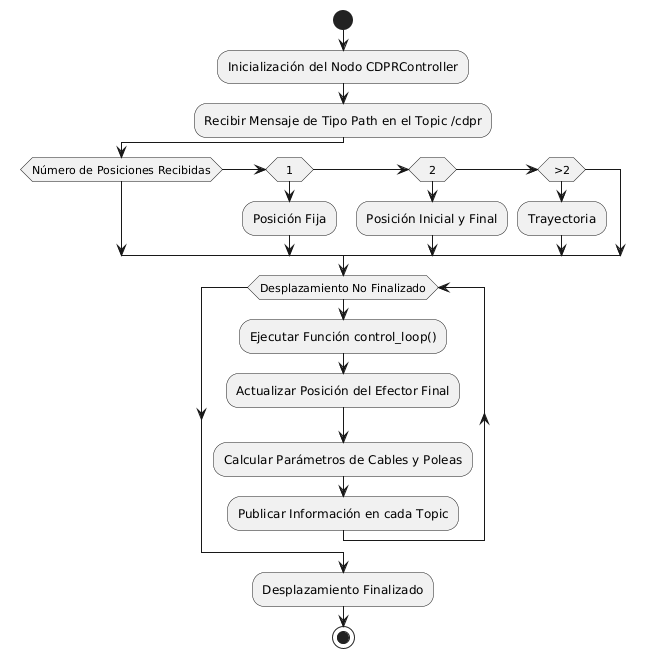
\includegraphics[width=\textwidth]{figs/general_system_workflow.png}
    \end{center}
    \caption{Flujo general de funcionamiento del sistema}
\end{figure}\

\newpage

Como se puede observar, el nodo recibe una única posición o una trayectoria objetivo, a partir de la cual se aplica el modelo cinemático para calcular la longitud de cada cable y los ángulos de rotación de cada polea.

\vspace{0.25cm}

Una vez hecho esto, el sistema publica los resultados obtenidos en topics, permitiendo así conocer el estado del sistema en tiempo real, al igual que en RViZ, donde se puede observar el movimiento del efector final y de las poleas en cada momento de la ejecución del sistema.

\section{Relación entre módulos}
\label{sec:segundaseccion}

Aunque gran parte de toda la funcionalidad del sistema se implemente en un único nodo, se pueden identificar claramente las relaciones entre todos los módulos que lo componen, como son las posiciones recibidas por su entrada, el cálculo cinemático y su visualización, lo que permite analizar y depurar el comportamiento del sistema de una forma mucho más estructurada, y que además, esta organización se puede seguir teniendo en cuenta en caso de que se quieran hacer ampliaciones en un futuro, como podría ser la adición de otro tipo de sensores en adición a los servomotores que ya se tienen, el paso de tener un sistema de control en lazo abierto a cerrado, o la separación del código en múltiples nodos ROS 2 en lugar de uno solo.


\chapter{Modelo cinemático}
\label{cap:capitulo4}

\vspace{0.25cm}

\section{Introducción}
\label{sec:segundaseccion}

El modelo cinemático constituye uno de los pilares fundamentales en el desarrollo del CDPR presentado en este TFG, cuyo objetivo principal es establecer una relación matemática entre la posición $(x,y)$ del efector final, la longitud de cada cable y los ángulos asociados a su orientación y accionamiento mediante poleas.

\vspace{0.25cm}

En este capítulo se presenta el modelo cinemático del sistema, tomando como referencia la implementación del mismo en el nodo ROS 2 desarrollado, cuyo enfoque es puramente geométrico y adecuado para un sistema de dos grados de libertad como el que se tiene y con el que se pueden describir perfectamente todos sus comportamientos.

\section{Descripción geométrica del sistema}
\label{sec:segundaseccion}

El sistema está formado por un efector final rígido, que se desplaza dentro de un plano bidimensional, suspendido mediante dos cables, cada uno de ellos conectado a una polea fija situada en cada una de las esquinas superiores de la estructura, las cuales se encuentran en posiciones ya conocidas dentro del marco de referencia global.

\vspace{0.25cm}

Sabiendo esto, se define un sistema de referencia cartesiano fijo $\{O\}$ asociado a la estructura del robot, donde el espacio de trabajo coincide con el plano $XY$. Por tanto, la posición del efector final se describe mediante el vector:

\begin{myequation}[h]
\begin{equation}
p = (x,y)
\end{equation}
\caption[Vector de posición del efector final]{Vector de posición del efector final}
\end{myequation}

\newpage

donde $x$ e $y$ representan las coordenadas del centro geométrico del efector final. Las dimensiones del efector final vienen definidas por un ancho $W_e$ y una altura $H_e$, donde los puntos de anclaje no coinciden con el centro del efector, sino con sus esquinas superiores.

\section{Definición de los puntos de anclaje}
\label{sec:segundaseccion}

Siendo $P_i=(X_i,Y_i)$ y $P_d=(X_d,Y_d)$ las posiciones de las poleas izquierda y derecha respectivamente, las cuales son parámetros ya conocidos y fijos en el sistema, se pueden definir los puntos de conexión de cada cable al efector final de la siguiente forma:

\begin{myequation}[h]
\begin{equation}
C_i = (X_{Ci}, Y_{Ci}) =
\left(x-\frac{W_e}{2},\, y+\frac{H_e}{2}\right) \qquad C_d = (X_{Cd}, Y_{Cd}) =
\left(x+\frac{W_e}{2},\, y+\frac{H_e}{2}\right)
\end{equation}
\caption[Puntos de anclaje entre cada cable y el efector final]{Puntos de anclaje entre cada cable y el efector final}
\end{myequation}

Esta definición refleja de forma directa la implementación real del sistema y permite incorporar explícitamente las dimensiones físicas del efector final en el modelo cinemático.

\section{Cinemática inversa}
\label{sec:segundaseccion}

La cinemática inversa de este sistema consiste en determinar las longitudes de los cables necesarias para situar al efector final en cada una de las posiciones $(x,y)$ por las que se quiere mover el efector final, donde las longitudes de los cables izquierdo y derecho respectivamente, se obtienen como la distancia euclídea entre cada polea y su correspondiente punto de conexión con el efector final de la siguiente forma:

\begin{myequation}[h]
\begin{equation}
L_i = \sqrt{(X_i - X_{Ci})^2 + (Y_i - Y_{Ci})^2} \qquad L_d = \sqrt{(X_d - X_{Cd})^2 + (Y_d - Y_{Cd})^2}
\end{equation}
\caption[Longitudes de cada cable]{Longitudes de cada cable}
\end{myequation}

En este modelo los cables se asumen como inextensibles y sin masa, resultando adecuado para el alcance que se le quiere dar a este TFG.

\newpage

\section{Cálculo de los ángulos de los cables}
\label{sec:segundaseccion}

Además de la longitud de cada cable, también es importante conocer el ángulo que forma cada cable con la vertical del sistema de referencia, los cuales se calculan de la siguiente forma:

\begin{myequation}[h]
\begin{equation}
\theta_i = \operatorname{arctan2}(Y_i - Y_{Ci},\, X_{Ci} - X_i) \qquad \theta_d = \operatorname{arctan2}(Y_d - Y_{Cd},\, X_{Cd} - X_d)
\end{equation}
\caption[Orientación angular de cada cable]{Orientación angular de cada cable}
\end{myequation}

En términos de software, los ángulos obtenidos en radianes se pasan a grados, de forma que puedan adaptarse lo mejor posible a la hora de visualizar el sistema en movimiento desde RViZ.

\section{Relación cables-poleas}
\label{sec:segundaseccion}

El accionamiento de los cables se realiza mediante el uso de dos poleas de radio $R_p$, lo que implica que un cambio en la longitud de uno de los cables se traduce directamente en una rotación de la polea correspondiente.

\vspace{0.25cm}

Siendo $\Delta$L la diferencia de longitud del cable entre dos posiciones consecutivas del efector final, el ángulo de rotación de la polea se puede obtener como:

\begin{myequation}[h]
\begin{equation}
\Delta\theta = \frac{\Delta L}{R_p}
\end{equation}
\caption[Relación entre desplazamiento y rotación de cada cable y polea]{Relación entre desplazamiento y rotación de cada cable y polea}
\end{myequation}

Por tanto, este modelo permite relacionar el espacio cartesiano del efector final con el espacio articular del sistema, definido por los ángulos de rotación de cada una de las poleas.

\newpage

\section{Consideraciones y limitaciones}
\label{sec:segundaseccion}

El modelo cinemático presentado puede considerarse como una versión simplificada, ya que siempre se tiene en cuenta que los cables nunca se verán afectados por ningún tipo de fuerza externa o porque éstos no poseen ningún tipo de propiedad elástica, además de la ausencia de fricción en las poleas.

\vspace{0.25cm}

Sin embargo, a pesar de estas simplificaciones, el modelo cinemático descrito recoge requisitos más que suficientes para describir el comportamiento general del sistema y demostrar que es válido tanto para realizar pruebas simuladas como reales, las cuales también deben tenerse en cuenta a la hora de plantear mejoras en un futuro.


\chapter{Simulación y validación del modelo}
\label{cap:capitulo5}

\vspace{0.25cm}

\section{Introducción}
\label{sec:segundaseccion}

Una vez desarrollado el modelo cinemático del CDPR, se ha llevado a cabo un proceso de validación y simulación con el objetivo de comprobar las expresiones matemáticas obtenidas del modelo cinemático en una primera implementación software. Esto permite verificar el comportamiento del sistema para así poder detectar posibles errores de planteamiento y evitar que se vayan acarreando a la hora de integrar el sistema completo en ROS 2.

\vspace{0.25cm}

En el caso de este TFG, las pruebas del modelo cinemático se han ido realizando de forma progresiva mediante su implementación en tres lenguajes de programación diferentes: MATLAB, Python y C++.

\section{Simulación inicial en MATLAB}
\label{sec:segundaseccion}

MATLAB es el primer lenguaje de programación que se ha utilizado para validar el modelo cinemático, ya que éste se considera idóneo para tratar expresiones matemáticas y obtener una rápida visualización de los resultados. Es por ello que, en esta fase inicial, la simulación se ha centrado exclusivamente en verificar que el efector final se ubica correctamente en una posición $(x,y)$ específica.

\vspace{0.25cm}

Esta primera implementación permite introducir directamente la posición $(x,y)$ en la que se quiere mostrar el efector final, además de ofrecer una representación gráfica de su posición exacta dentro del espacio de trabajo junto con toda la estructura del sistema y la disposición de los cables. 

\begin{figure} [h!]
    \begin{center}
        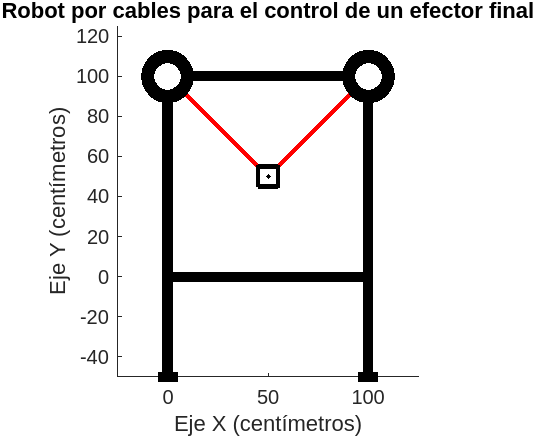
\includegraphics[width=0.5\textwidth]{figs/matlab_kinematic_model.png}
    \end{center}
    \caption{Simulación inicial en MATLAB}
\end{figure}\

\newpage

Con esto se ha cumplido el objetivo de esta primera versión, que no comprende la simulación del movimiento del efector final ni la planificación de trayectorias, sino que lo que se busca es verificar que el modelo cinemático sitúe al efector final en la posición deseada y que las longitudes de los cables calculadas sean coherentes con la geometría del sistema, sirviendo así como validación conceptual del modelo y como punto de partida para implementaciones posteriores.

\section{Implementación del modelo en Python}
\label{sec:segundaseccion}

Una vez validado el primer modelo en MATLAB, se ha desarrollado una implementación más avanzada en Python, la cual ya incluye animaciones y la posibilidad de definir múltiples posiciones objetivo para así generar trayectorias contínuas que conecten dichos puntos.

\vspace{0.25cm}

Esta segunda implementación permite introducir una secuencia de posiciones objetivo para el efector final dentro del espacio de trabajo. A partir de estas posiciones, se pueden interpolar trayectorias rectilíneas entre puntos consecutivos, mientras se calculan en cada instante las longitudes y los ángulos de cada cable utilizando las ecuaciones correspondientes de cinemática inversa.

\newpage

Además, esta implementación incluye una representación gráfica del sistema, en la que se muestra la estructura, la trayectoria realizada, y la variación del movimiento del efector final y los cables en todo momento, facilitando así la comprensión del funcionamiento del sistema y permitiendo observar de forma intuitiva cómo va evolucionando el movimiento del efector final y de los cables. Es por ello que esta segunda versión ya se aproxima mucho más al funcionamiento que se implementará posteriormente en ROS 2.

\vspace{0.25cm}

Para una mejor comprensión del comportamiento dinámico del sistema mostrado en la figura, se adjunta un enlace de descarga a un vídeo demostrativo al que se puede acceder haciendo clic \href{https://github.com/aleon2020/cable_driven_parallel_robot_2d/raw/refs/heads/main/media/gifs/python_kinematic_model_v3_execution.gif}{aquí}.

\begin{figure} [h!]
    \begin{center}
        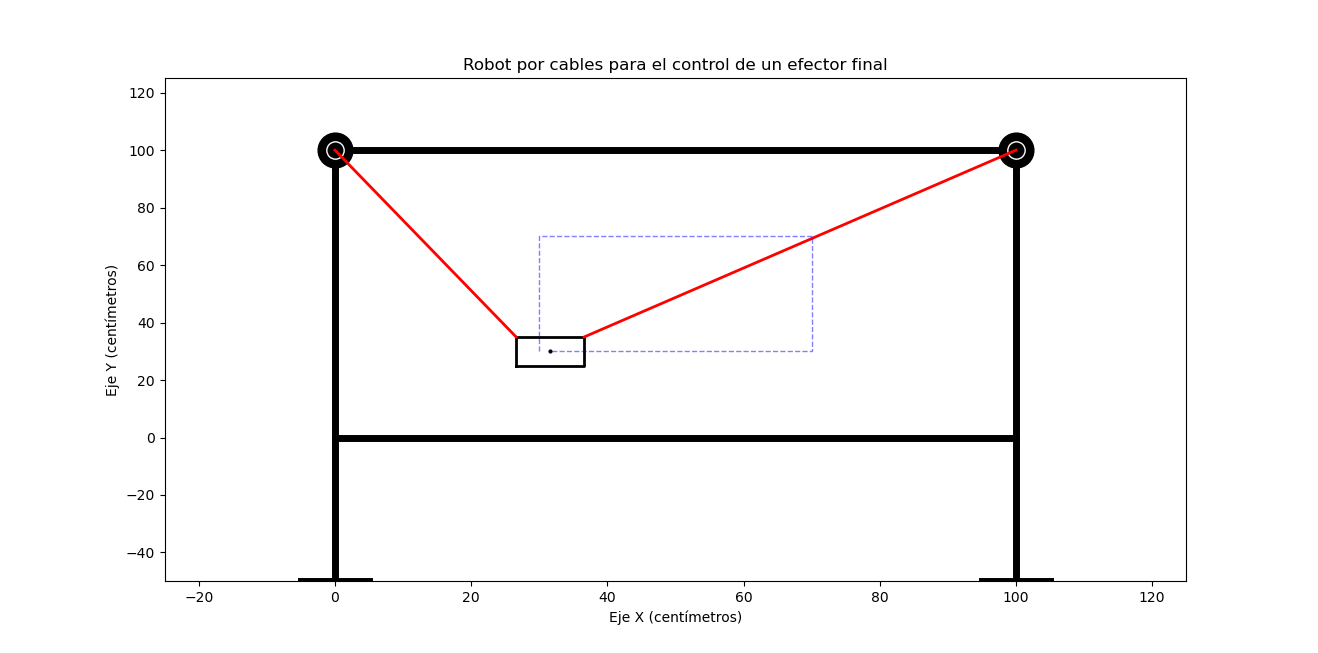
\includegraphics[width=0.5\textwidth]{figs/python_kinematic_model_v3.png}
    \end{center}
    \caption{Implementación y simulación en Python}
\end{figure}\

\section{Implementación del modelo en C++}
\label{sec:segundaseccion}

En paralelo a la implementación en Python, se ha desarrollado una versión del modelo cinemático en C++. Esta implementación reproduce la misma lógica que la vista en Python, permitiendo la definición de varias posiciones objetivo y el cálculo de la longitud de los cables en cada momento para recorrer una trayectoria.

\vspace{0.25cm}

Esta simulación se ha llevado a cabo únicamente con fines de verificación y comparación para asegurar que el modelo cinemático es independiente del lenguaje de programación utilizado, y que todas las ecuaciones que lo forman sean consistentes. Y aunque la visualización gráfica en C++ no sea tan completa como la de Python, también es útil para validar todos los cálculos numéricos realizados.

\vspace{0.25cm}

Para una mejor comprensión del comportamiento dinámico del sistema mostrado en la figura, se adjunta un enlace de descarga a un vídeo demostrativo al que se puede acceder haciendo clic \href{https://github.com/aleon2020/cable_driven_parallel_robot_2d/raw/refs/heads/main/media/gifs/cpp_kinematic_model_v3_execution.gif}{aquí}.

\begin{figure} [h!]
    \begin{center}
        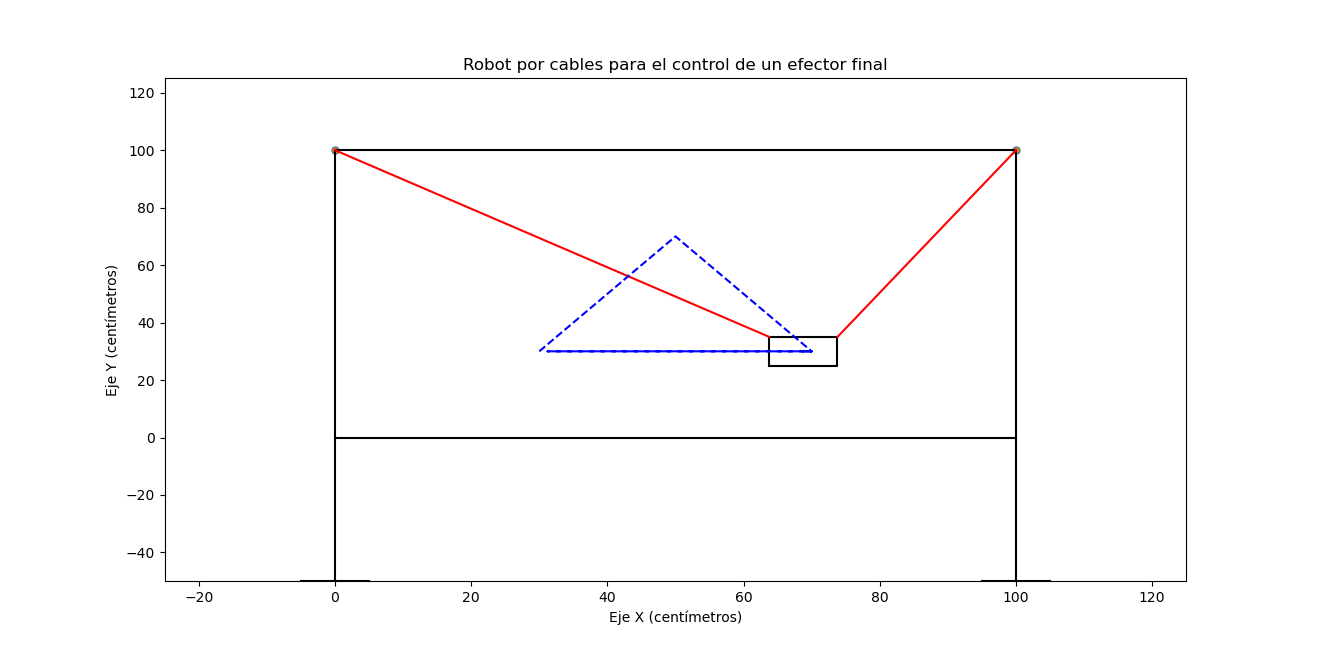
\includegraphics[width=0.5\textwidth]{figs/cpp_kinematic_model_v3.png}
    \end{center}
    \caption{Implementación y simulación en C++}
\end{figure}\

\section{Comparación y validación de resultados}
\label{sec:segundaseccion}

Para validar el modelo cinemático, se han comparado los resultados obtenidos en las tres implementaciones, y todas ellas presentan una muy buena concordancia, lo que deja más que confirmado que el modelo cinemático utilizado es totalmente correcto.

\vspace{0.25cm}

Sin embargo, existen algunas diferencias en cuanto a funcionalidad y flexibilidad. MATLAB se ha utilizado como herramienta para llevar a cabo una primera validación, limitándose únicamente al posicionamiento de una única posición objetivo, mientras que las implementaciones realizadas en Python y en C++ permiten la generación de trayectorias definidas por múltiples posiciones objetivo.

\vspace{0.25cm}

Y es por eso que, tras este análisis comparativo, he decidido utilizar Python como lenguaje principal a la hora de implementar el sistema en ROS 2, debido a la facilidad que supone desarrollar en Python ofreciendo la posibilidad de poder integrarlo directamente en ROS 2, manteniendo el mismo comportamiento cinemático que en C++.

\section{Análisis de errores y limitaciones}
\label{sec:segundaseccion}

Durante el proceso de simulación, se han identificado algunas limitaciones que no afectan al sistema debido al enfoque que se le ha dado al mismo, ya que al tratarse de un modelo puramente cinemático, no se consideran efectos dinámicos como la masa del efector final, la elasticidad de los cables o la fricción de las poleas.

\vspace{0.25cm}

Por otro lado, todas las simulaciones se realizan en lazo abierto, lo que implica que todos los resultados obtenidos dependen directamente de la precisión del modelo y de los parámetros geométricos definidos. Todas estas limitaciones no invalidan ningún aspecto del sistema ya definido, pero es importante tenerlas en cuenta a la hora de interpretar los resultados cuando se esté implementando en un entorno físico real.


\chapter{Integración del sistema en ROS 2}
\label{cap:capitulo6}

\section{Introducción}
\label{sec:segundaseccion}

Una vez validado el modelo cinemático del CDPR en todas las simulaciones mencionadas en el capítulo anterior, el siguiente paso consiste en la integración completa del sistema en ROS 2 \cite{ros2_docs}, lo que va a permitir dotar al sistema de una arquitectura modular y escalable, facilitando así su visualización a la hora de probarlo en un sistema físico real.

\vspace{0.25cm}

En este capítulo se describe la estructura general de los paquetes de ROS 2 \cite{ros2_docs} desarrollados, el funcionamiento del nodo que implementa toda la parte de control del CDPR, todo lo relacionado con las comunicaciones realizadas mediante topics y servicios, y la visualización del sistema en RViZ \cite{rviz_docs}.

\vspace{0.25cm}

Toda esta integración se ha llevado a cabo haciendo uso de la distribución Jazzy de ROS 2 \cite{ros2_docs} y de Python como lenguaje de programación, tal y como se mencionó en el capítulo anterior.

\newpage

\section{Estructura de los paquetes}
\label{sec:segundaseccion}

\begin{code}[h]
\begin{lstlisting}
src
|-- cdpr_2d
|   |-- cdpr_controller.py
|   |-- config (RViZ)
|   |-- description (URDF)
|   `-- robot_state_publisher.launch.py
|
|-- cdpr_figures
|   |-- figures_library.py
|   `-- figures_service.py
|
`-- cdpr_interfaces
    `-- DrawFigure.srv
\end{lstlisting}
\caption[Estructura del workspace ROS 2.]{Estructura del workspace ROS 2.}
\end{code}

Esta organización del workspace permite distinguir claramente de qué tareas se encarga cada uno de los paquetes que lo componen. \textit{cdpr\_2d} implementa el controlador principal del sistema y todos los ficheros necesarios para su simulación y validación en RViZ \cite{rviz_docs}, \textit{cdpr\_figures} contiene una librería que permite generar trayectorias asociadas a letras, números, polígonos y otras figuras geométricas, y por último, \textit{cdpr\_interfaces} define las interfaces de comunicación haciendo uso de servicios.

\vspace{0.25cm}

Por tanto, esta separación facilita el mantenimiento del código y hace que sea más sencillo añadir nuevas funcionalidades y componentes sin necesidad de tener que reestructurar todo el workspace.

\section{Arquitectura interna del nodo principal de control}
\label{sec:segundaseccion}

El sistema integrado en ROS 2 \cite{ros2_docs} tiene como núcleo el nodo \textit{cdpr\_controller}, encargado de recibir las posiciones objetivo por las que se quiere desplazar el efector final para así poder aplicarlas en el modelo cinemático desarrollado, con el objetivo de obtener todos los parámetros relacionados con los cables y las poleas del sistema.

\vspace{0.25cm}

El nodo se inicializa y se mantiene activo en todo momento para que pueda recibir todos los mensajes que contienen cada una de las posiciones objetivo, simplificando la integración y el análisis del sistema completo.

\begin{figure} [h!]
    \begin{center}
        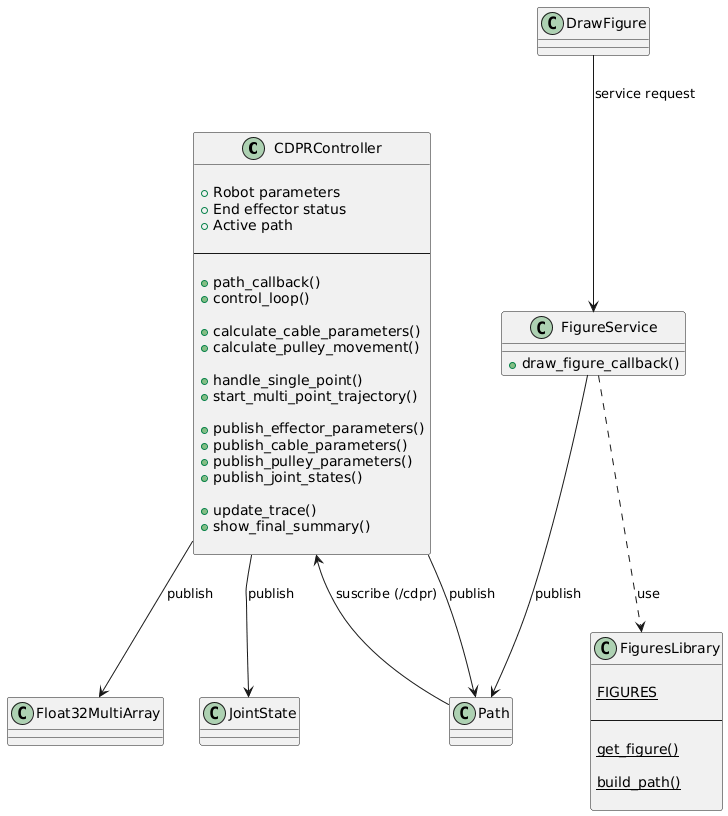
\includegraphics[width=\textwidth]{figs/class_diagram.png}
    \end{center}
    \caption{Diagrama UML de las clases que componen toda la arquitectura software desarrollada. En él se representan el controlador principal, el servicio encargado de generar figuras y la librería en la que se encuentran todas ellas predefinidas, además de las relaciones existentes entre todos los componentes mediante mensajes y servicios de ROS 2.}
\end{figure}\

Como se puede observar, la clase principal corresponde al nodo \textit{cdpr\_controller}, encargado de gestionar la ejecución del sistema dentro de ROS 2 \cite{ros2_docs}.

\newpage

Este nodo recibe todas las posiciones objetivo por las que se quiere desplazar el efector final haciendo uso del modelo cinemático para calcular todos los parámetros asociados a los cables y a las poleas, para posteriormente, publicar toda esta información en distintos topics.

\vspace{0.25cm}

Es por ello que esta organización es la que permite concentrar gran parte de la lógica del sistema en un único nodo principal, siguiendo una estructura que facilita la comprensión del mismo, y donde podrían llevarse a cabo ampliaciones en un futuro.

\vspace{0.25cm}

Para una mejor comprensión del comportamiento dinámico del sistema mostrado en la figura, se adjunta un enlace a un vídeo demostrativo al que se puede acceder haciendo clic \href{https://github.com/aleon2020/cable_driven_parallel_robot_2d/raw/refs/heads/main/media/gifs/3_or_more_points_execution.gif}{aquí}.

\begin{figure} [h!]
    \begin{center}
        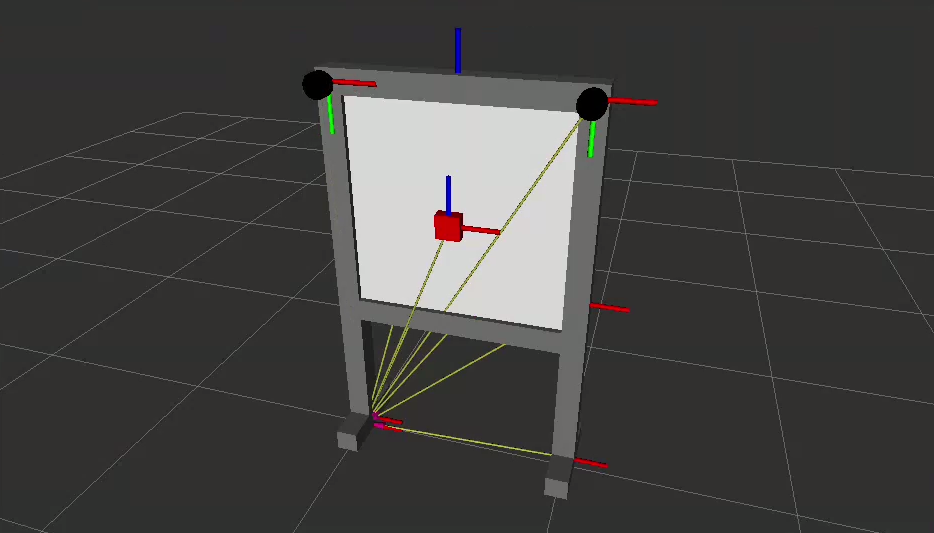
\includegraphics[width=\textwidth]{figs/cable_driven_parallel_robot.png}
    \end{center}
    \caption{Visualización en RViZ durante la ejecución de una trayectoria. En esta imagen se puede observar la estructura fija del CDPR en gris, el espacio de trabajo del efector final en blanco, las poleas en negro, y al propio efector final en rojo, mientras que en el vídeo adjunto se puede visualizar la evolución del movimiento del efector final y de las poleas conforme se actualiza el estado publicado por el nodo de control, lo que permite verificar si el comportamiento del sistema es correcto.}
\end{figure}\

\newpage

\section{Comunicación mediante topics}
\label{sec:segundaseccion}

La comunicación entre el nodo \textit{cdpr\_controller} y el resto del sistema se lleva a cabo utilizando topics que siguen un modelo publicador-suscriptor, lo que permite diferenciar los distintos componentes del sistema y monitorear el estado del mismo en tiempo real.

\vspace{0.25cm}

Por ello, se adjunta a continuación un diagrama de secuencia que muestra el intercambio de mensajes y cómo se produce esta comunicación entre los distintos componentes del sistema.

\begin{figure} [h!]
    \begin{center}
        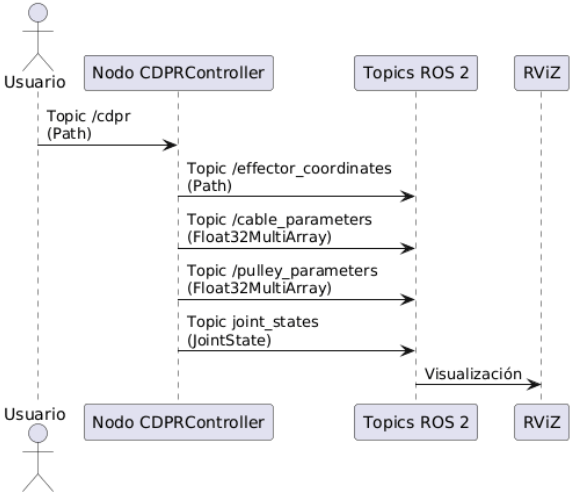
\includegraphics[width=\textwidth]{figs/communication_via_topics.png}
    \end{center}
    \caption{Grafo de comunicación que representa los nodos y topics utilizados durante la ejecución del sistema, donde se muestra el intercambio de información entre el controlador principal, los topics y las herramientas de visualización como lo es RViZ en este caso, facilitando así la comprensión del flujo de datos y las comunicaciones del sistema.}
\end{figure}\

\newpage

En primer lugar, el usuario publica una única posición o un conjunto de posiciones objetivo en el topic correspondiente. Después, el nodo \textit{cdpr\_controller} recibe este mensaje y va procesando cada una de las posiciones objetivo que ha recibido haciendo uso del modelo cinemático. Y por último, el nodo \textit{cdpr\_controller} publica en cada topic correspondiente mensajes sobre la posición del efector final o parámetros asociados a los cables y a las poleas, los cuales son también utilizados por RViZ \cite{rviz_docs} para poder representar el estado del sistema de forma visual y en tiempo real.

\section{Gestión de trayectorias y movimientos}
\label{sec:segundaseccion}

Además del paquete que contiene el nodo correspondiente al controlador principal (\textit{cdpr\_2d}), el sistema incluye un paquete llamado \textit{cdpr\_figures} que contiene una biblioteca de figuras predefinidas y se encarga de ofrecer servicios para su ejecución. Y por último, el paquete \textit{cdpr\_interfaces} define las interfaces de comunicación utilizadas como servicios personalizados. Es por ello que esta separación hace más sencilla la reutilización del código, resultando así en una arquitectura modular y escalable.

\vspace{0.25cm}

Este sistema tiene implementados diferentes modos de comportamiento en función del número de puntos recibidos en el mensaje de tipo \textit{nav\_msgs/msg/Path} \cite{nav_msgs_path}.

\vspace{0.25cm}

Cuando se recibe una única posición, el sistema interpreta la posición recibida como un posicionamiento fijo del efector final. En caso de haber recibido dos posiciones, se genera un desplazamiento entre una posición inicial y una posición final. Y por último, si se reciben tres o más posiciones, el sistema lo interpreta como una trayectoria compuesta por todas las posiciones que se le han pasado y por las que el efector final debe pasar en el orden especificado.

\vspace{0.25cm}

Para este último caso, el nodo interpola posiciones intermedias y aplica el modelo cinemático para calcular los parámetros correspondientes en todo momento para cada segmento de la trayectoria. Esto permite simular un movimiento contínuo y coherente del efector final dentro del espacio de trabajo.

\section{Visualización del sistema en RViZ}
\label{sec:segundaseccion}

La integración del sistema y su visualización en RViZ \cite{rviz_docs} son claves en el desarrollo del mismo, ya que permiten observar de forma mucho más clara el comportamiento del sistema. Para ello, se ha definido un modelo URDF \cite{urdf_docs} que describe la estructura fija, los cables, las poleas y el efector final.

\vspace{0.25cm}

El lanzamiento conjunto de los nodos \textit{cdpr\_controller} y \textit{robot\_state\_publisher} permiten actualizar en todo momento la visualización del robot en RViZ \cite{rviz_docs} según se va ejecutando cada trayectoria, cuya configuración facilita la observación de los distintos elementos que componen el sistema y su evolución cuando se encuentran en movimiento.

\section{Compilación y ejecución del sistema}
\label{sec:segundaseccion}

Con el objetivo de reproducir todo el trabajo desarrollado, se ha elaborado una \href{https://github.com/aleon2020/cable_driven_parallel_robot_2d/blob/main/README.md}{guía de ejecución} que enumera todos los pasos necesarios para compilar el workspace \cite{colcon_docs}, inicializar todos los nodos y poner en funcionamiento el sistema completo. Sin embargo, para no opacar la memoria con comandos u otras instrucciones de este tipo, dicha guía se incluye en el \href{https://github.com/aleon2020/cable_driven_parallel_robot_2d}{repositorio de GitHub oficial} de este proyecto.

\vspace{0.25cm}

La principal ventaja de trasladar toda esta información a un repositorio de GitHub \cite{github_docs,tfg_repository,microros_espidf,microxrce_dds} externo es que permite centrar la memoria en todos los aspectos relacionados con el diseño e implementación del sistema, además de proporcionar a quien la esté leyendo una referencia práctica para poder ejecutar todas las pruebas realizadas y utilizar el sistema completo desarrollado, facilitando así futuras modificaciones de los procesos de instalación y ejecución sin afectar a la estructura de la memoria.

\vspace{0.25cm}

Como inconveniente, la consulta de los pasos de instalación y ejecución del sistema requieren acceder a material externo a la memoria. Sin embargo, esta separación permite distinguir claramente entre la descripción técnica del sistema y las instrucciones necesarias para su ejecución.


\chapter{Desarrollo hardware}
\label{cap:capitulo7}

\vspace{0.25cm}

\section{Introducción}
\label{sec:segundaseccion}

...

\section{Diseño mecánico del sistema}
\label{sec:segundaseccion}

...

\section{Sistema electrónico}
\label{sec:segundaseccion}

...

\section{Programación del microcontrolador}
\label{sec:segundaseccion}

...

\section{Integración hardware-software}
\label{sec:segundaseccion}

...

\section{Consideraciones prácticas y limitaciones del prototipo}
\label{sec:segundaseccion}

...

\section{Resumen}
\label{sec:segundaseccion}

...

\clearpage
\thispagestyle{empty}

\printindex \nocite{*}
\appendix
\bibliographystyle{unsrt} \bibliography{bibliografia}

\end{document}
